\section{Stream Ciphers --- LFSR Sequences}\label{sec:Stream_Ciphers}
There are 2 main types of \nameref{def:Symmetric_Encryption} algorithms:
\begin{enumerate}[noitemsep]
\item \nameref{def:Block_Cipher}s
\item \nameref{def:Stream_Cipher}s
\end{enumerate}

\begin{definition}[Block Cipher]\label{def:Block_Cipher}
  \emph{Block cipher}s encrypt a block of symbols of a fixed size from the \nameref{def:Plaintext} message using an fixed-size encryption transformation.
\end{definition}

\begin{definition}[Stream Cipher]\label{def:Stream_Cipher}
  \emph{Stream cipher}s encrypt individual characters of the \nameref{def:Plaintext} using an encryption transofrmation that varies with time.
  The 2 elements that make up a stream cipher are \textbf{memory} and a \textbf{combinatorial function}.
  \begin{enumerate}[noitemsep]
  \item Memory
    \begin{itemize}[noitemsep]
    \item \nameref{def:LFSR}s
    \item Tables (Arrays)
    \end{itemize}
  \item Combinatorial Function
    \begin{itemize}[noitemsep]
    \item Nonlinear Boolean functions, S-boxes
    \item XOR, Modular addition, cyclic rotations, multiplication
    \end{itemize}
  \end{enumerate}
\end{definition}

\begin{definition}[Keystream]\label{def:Keystream}
  The \emph{keystream} is the output of the generator, which gets used on the \nameref{def:Plaintext} message to form the \nameref{def:Ciphertext}
  \begin{equation}\label{eq:Keystream}
    \mathbf{z} = z_{1}, z_{2}, \ldots
  \end{equation}

  \begin{remark}[Attacks]\label{rmk:Keystream_Attack_Vectors}
    For a synchronous \nameref{def:Stream_Cipher}, a \nameref{def:Attack-Known_Plaintext}, \nameref{def:Attack-Chosen_Plaintext}, or \nameref{def:Attack-Chosen_Ciphertext} is equivalent to having access to the \nameref{def:Keystream}.
  \end{remark}

  \begin{remark}[Secret Key]\label{rmk:Keystream_Secret_Key}
    When the \nameref{def:Keystream} first starts, because it is a synchronous system, it needs to have a starting value with which to generate subsequent values.
    This first value may be fixed, and is the secret key, $K$, in this case.
  \end{remark}
\end{definition}

\subsection{Assumptions}\label{subsec:Stream_Cipher_Assumptions}
We assume that
\begin{itemize}[noitemsep]
\item The output \nameref{def:Keystream} of length $N$ is known to Eve.
\end{itemize}

\subsection{Attacks}\label{subsec:Stream_Cipher_Attacks}
An attack is considered successful only if the complexity of performing it is considerably lower than the exhaustive keysearch of complexity $2^{k}$.

The attack types that are of interest are:
\begin{itemize}[noitemsep]
\item \emph{\nameref{def:Attack-Key_Recovery}}: Eve tries to recover the \nameref{rmk:Keystream_Secret_Key}, $K$.
\item \emph{\nameref{def:Attack-Distinguishing}}: Eve tries to determine whether a given sequence $\hat{\mathbf{z}} = z_{1}, z_{2}, \ldots, z_{N}$ is likely to have been generated from the considered \nameref{def:Stream_Cipher}, or if it's a truly random sequence.
\end{itemize}

\begin{definition}[Key Recovery Attack]\label{def:Attack-Key_Recovery}
  In a \emph{key recovery attack}, Eve tries to recover the \nameref{rmk:Keystream_Secret_Key}, $K$.
\end{definition}

\begin{definition}[Distinguishing Attack]\label{def:Attack-Distinguishing}
  In a \emph{distinguishing attack}, Eve tries to determine whether a given sequence $\hat{\mathbf{z}} = z_{1}, z_{2}, \ldots, z_{N}$ is likely to have been generated from the considered \nameref{def:Stream_Cipher}, or if it's a truly random sequence.

  Let $D(\mathbf{z})$ be an algorithm that takes in a sequence $\mathbf{z}$ of length $N$, and outputs either ``X'' or ``RANDOM''.
  With probability $\frac{1}{2}$, the sequence $\mathbf{z}$ is produced by a generator $X$ otherwise, it is a random sequence.
  The probability that $D(\mathbf{z})$ correctly determines the origin of $\mathbf{z}$ is written $\Prob \bigl( D(\mathbf{z}) \bigr) = \frac{1}{2} + \epsilon$.
  If $\epsilon$ is not very close to zero, then $D(\mathbf{z})$ is a \emph{distinguisher} for the generator $X$, because it can more often than not distinguish that the sequence is nonrandom.

  \begin{remark}
    A \nameref{def:Attack-Distinguishing} is a much weaker attack than a \nameref{def:Attack-Key_Recovery}.
  \end{remark}
\end{definition}

\subsection{Linear Feedback Shift Registers}\label{subsec:LFSRs}
\begin{definition}[Linear Feedback Shift Register]\label{def:LFSR}
  A \emph{linear feedback shift register} is a data storage element.
  A register has $L$ delay (storage) elements, each of which is capable of storing one element from the field \TextFiniteMathField{F}{q}{}, and a clock signal.
  When the clock signal is applied, the register's delay elements are shifted one step, and the value shifted into the beginning is calculated as a linear function of the contents of the register.

  \begin{figure}[h!]
    \centering
    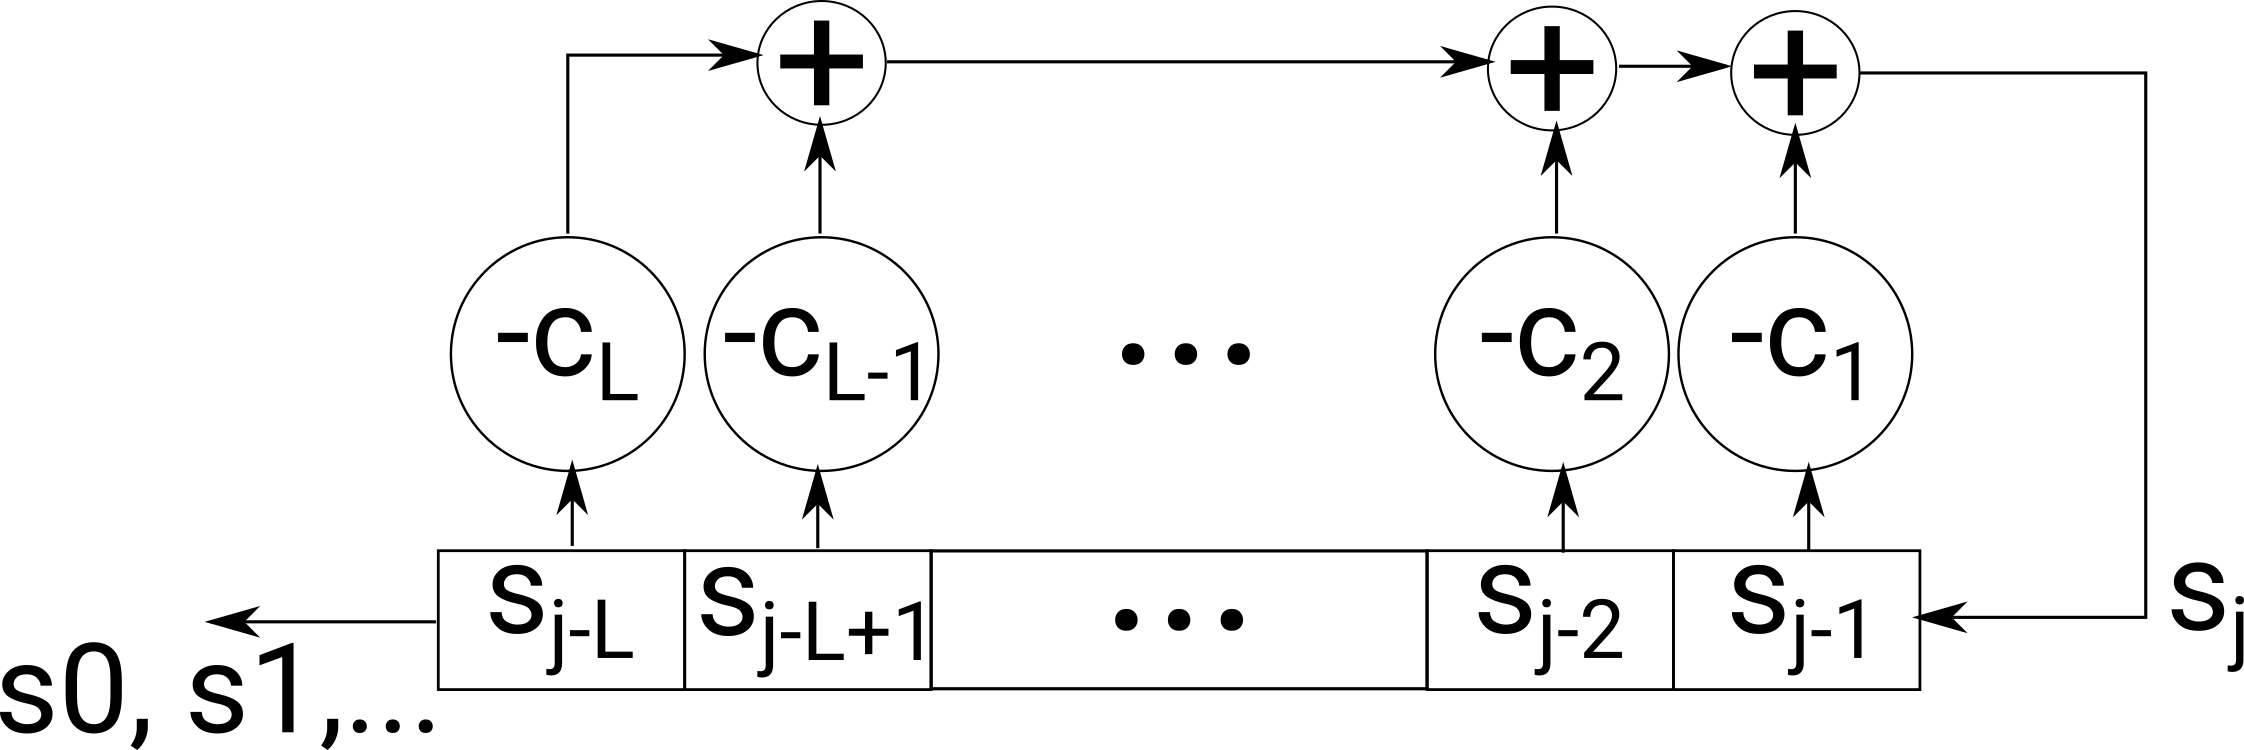
\includegraphics[scale=0.50]{./Drawings/EDIN01-Cryptography/Linear_Feedback_Shift_Register.png}
    \caption{\nameref{def:LFSR}}
    \label{fig:LSFR}
  \end{figure}
\end{definition}

\begin{definition}[Shift Register Equation]\label{def:Shift_Register_Equation}
  The \emph{shift register equation} is a way of describing the coefficients, $c_{1}, c_{2}, \ldots, c_{L} \in \FiniteMathField{F}{q}{}$, and their recurrence relation
  \begin{equation}\label{eq:Shift_Register_Equation}
    s_{j} = -c_{1}s_{j-1} - c_{2}s_{j-2} - \cdots - c_{L}s_{j-L}
  \end{equation}
  for $j = L, L+1, \ldots$.

  If  $c_{0} = 1$, we can write
  \begin{equation}\label{eq:Shift_Register_Equation-Summation}
    \sum\limits_{i=0}^{L} c_{i}s_{j-i} = 0, \text{ for } j = L, L+1, \ldots
  \end{equation}

  \begin{remark}[Initial State]\label{rmk:Shift_Register_Initial_State-Fibonacci}
    The first $L$ symbols, $s_{0}, s_{1}, \ldots, s_{L-1}$ form the \emph{initial state}.
  \end{remark}

  \begin{remark}[Fibonacci Implementation]\label{rmk:Shift_Register-Fibonacci}
    The \nameref{def:LFSR} setup shown in \Cref{fig:LSFR} is implemented in a \emph{fibonacci}-style.
  \end{remark}
\end{definition}

\begin{definition}[Connection Polynomial]\label{def:Connection_Polynomial}
  The coefficients, $c_{0}, c_{1}, \ldots, c_{L}$ are summarized in the \emph{connection polynomial}.
  \begin{equation}\label{eq:Connection_Polynomial}
    C(D) = 1 + c_{1}D + c_{2}D^{2} + \cdots + c_{L}D^{L}
  \end{equation}

  \begin{remark}[Alternate Form]\label{rmk:Connection_Polynomial-Alternate_Form}
    We can write the \nameref{def:Connection_Polynomial} in a slightly different form, to denote both the \nameref{def:Connection_Polynomial} and the length.
    \begin{equation}\label{eq:Connection_Polynomial-Alternate_Form}
      \langle C(D), L \rangle
    \end{equation}
  \end{remark}
\end{definition}

\begin{definition}[D-Transform]\label{def:D_Transform}
  The \emph{D-Transform} is actually just the $\mathcal{Z}$-Transform, with a different indeterminate variable.
  The D-transform of a sequence $\mathbf{s} = s_{0}, s_{1}, \ldots$ is defined as
  \begin{equation}\label{eq:D_Transform_Sequence}
    S(D) = s_{0} + s_{1}D + s_{2}D^{2}
  \end{equation}
  if $s_{i} \in \FiniteMathField{F}{q}{}$.

  The indeterminate $D$ is the ``delay'', and the exponent indicates the number of delays.

  \begin{remark}[Our Assumptions]
    For this course, we assume that $s_{i} = 0$ for $i < 0$, i.e.\ the signal is causal.
    The set of all such sequences having the form
    \begin{equation*}
      f(D) = \sum\limits_{i=0}^{\infty} f_{i}D^{i}
    \end{equation*}
    where $f_{i} \in \FiniteMathField{F}{q}{}$ is denoted \TextFiniteMathField{F}{q}{}[[D]], and is called the \emph{ring of formal power series}.
  \end{remark}
\end{definition}

\begin{theorem}\label{thm:D_Transform_Connection_Polynomial_Relation}
  The set of sequences generated by the \nameref{def:LFSR} with \nameref{def:Connection_Polynomial} $C(D)$ is the set of sequences that have the \nameref{def:D_Transform}
  \begin{equation}\label{eq:D_Transform_Sequence_Connection_Polynomial_Relation}
    S(D) = \frac{P(D)}{C(D)}
  \end{equation}
  where $P(D)$ is an arbitrary \nameref{def:Polynomial} of \nameref{def:Polynomial_Degree} at most $L-1$,
  \begin{equation}\label{eq:P_Polynomial}
    P(D) = p_{0} + p_{1}D + \cdots + p_{L-1}D^{L-1}
  \end{equation}

  The relation between the initial state of the \nameref{def:LFSR} and the $P(D)$ \nameref{def:Polynomial} is given by the linear relation.
  \begin{equation*}
    \begin{pmatrix}
      p_{0} \\
      p_{1} \\
      \vdots \\
      p_{L-1}
    \end{pmatrix}
     =
     \begin{pmatrix}
       1 & 0 & \cdots & 0 \\
       c_{1} & 1 & \cdots & 0 \\
       \vdots & \vdots & \ddots & \vdots \\
       c_{L-1} & c_{L-2} & \cdots & 1
     \end{pmatrix}
     \begin{pmatrix}
       s_{0} \\
       s_{1} \\
       \vdots \\
       s_{L-1}
     \end{pmatrix}
  \end{equation*}
\end{theorem}

\subsection{\nameref*{subsec:LFSRs} Sequences and Extension Fields}\label{LFSR_Sequences_Extension_Fields}
Let $\pi(x)$ be an \nameref{def:Irreducible_Polynomial} \nameref{def:Polynomial} over \TextFiniteMathField{F}{q}{} and assume its coefficients are
\begin{equation}\label{eq:Reciprocal_Connection_Polynomial}
  \pi(x) = x^{L} + c_{1}x^{L-1} + \cdots + c_{L}
\end{equation}
This means that $\pi(x)$ is the \emph{reciprocal} \nameref{def:Polynomial} of the \nameref{def:Connection_Polynomial} $C(D)$.

We can construct an \nameref{rmk:Extension_Field} \TextFiniteMathField{F}{q}{L} through $\pi(\alpha) = 0$.
The term $\beta$ from \TextFiniteMathField{F}{q}{} can be expressed in a \nameref{def:Polynomial} basis as
\begin{equation}\label{eq:Extension_Field-Beta}
  \beta = \beta_{0} + \beta_{1}\alpha^{1} + b_{2}\alpha^{2} + \cdots + \beta_{L-1} + \alpha^{L-1}
\end{equation}
where $\beta_{0}, \beta_{1}, \ldots, \beta_{L-1} \in \FiniteMathField{F}{q}{}$.

If we multiply \Cref{eq:Extension_Field-Beta} by $\alpha$, we get
\begin{equation*}
  \alpha\beta = \beta_{0}\alpha + \beta_{1}\alpha^{2} + \cdots + \beta_{L-1}\alpha^{L}
\end{equation*}
Now, we can reduce the $\alpha^{L}$ according to the $\pi(\alpha)=0$ relation we found earlier.
This gives us
\begin{equation}\label{eq:LFSR_Galois_Equation}
  \alpha\beta = -c_{L}\beta_{L-1} + \left( \beta_{0} - c_{L-1}\beta_{L-1} \right) \alpha + \cdots + \left( \beta_{L-2} - c_{1}\beta_{L-1} \right) \alpha^{L-1}
\end{equation}

\begin{figure}[h!]
  \centering
  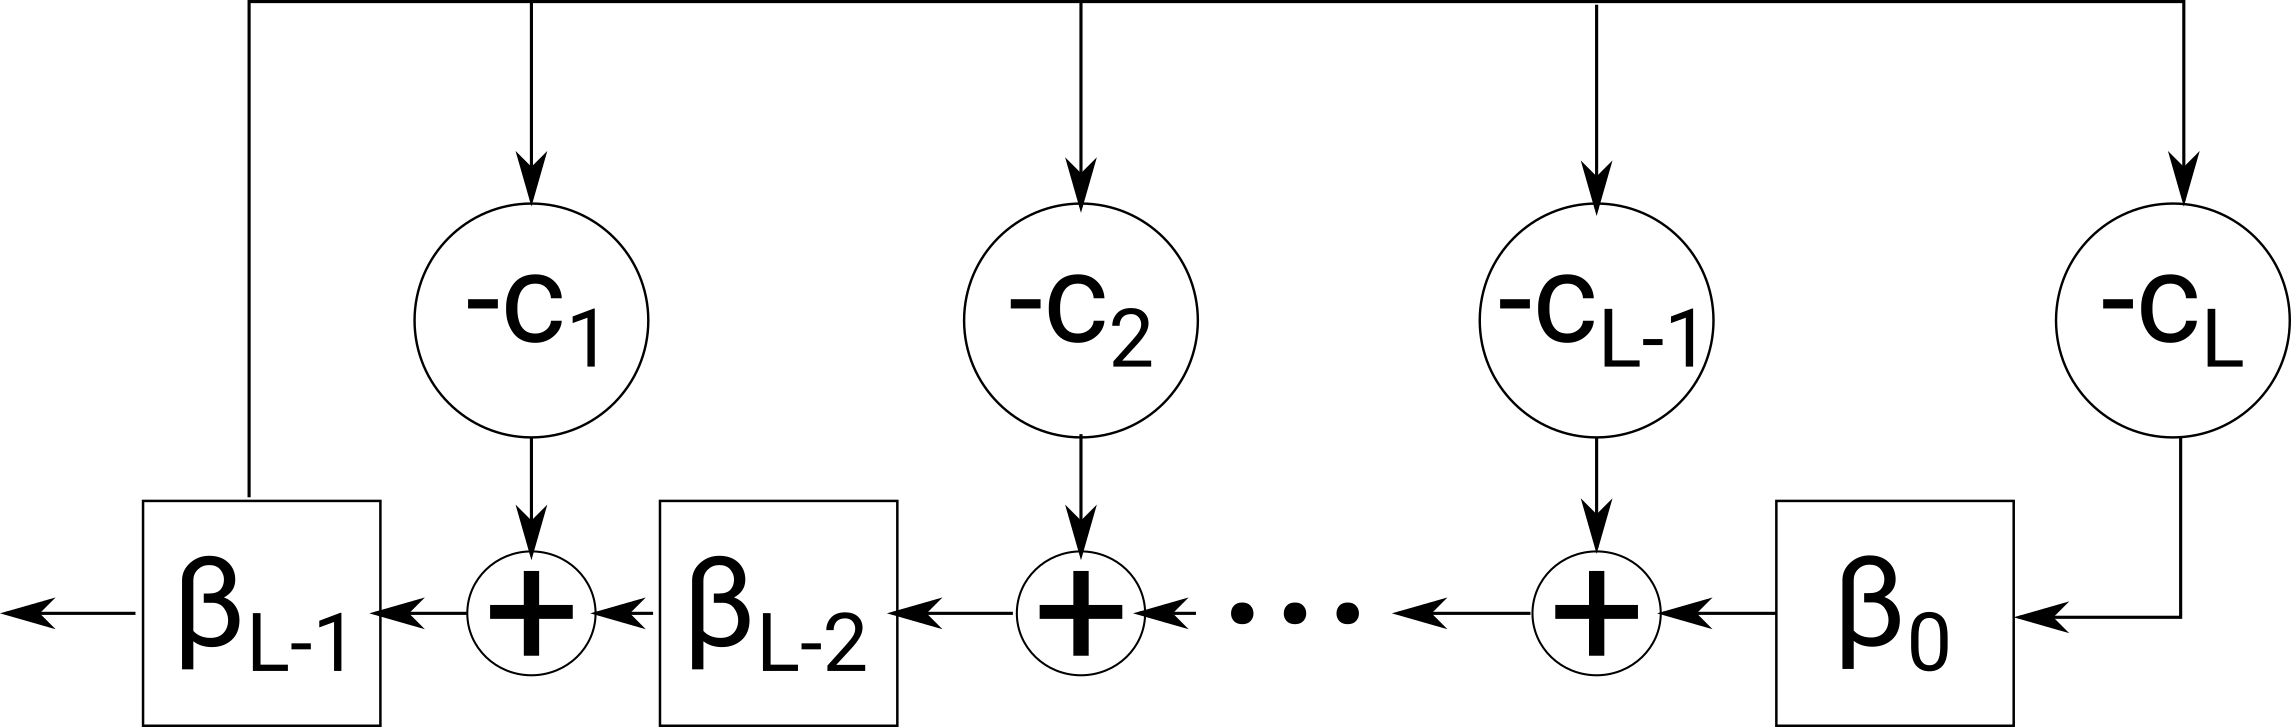
\includegraphics[scale=0.5]{./Drawings/EDIN01-Cryptography/Linear_Feedback_Shift_Register-Galois.png}
  \caption{\nameref{def:LFSR} in Galois Form}
  \label{fig:LFSR_Galois}
\end{figure}

We can check that this form, the \emph{Galois Form} of this \nameref{def:LFSR} is the same as the other.
\begin{equation*}
  s_{j} = -c_{1}s_{j-1} - c_{2}s_{j-2} - \cdots - c_{L}s_{j-L}
\end{equation*}
when $j \geq L$.
Also,
\begin{equation*}
  p_{0} = s_{0}, p_{1} = s_{1} + c_{1}s_{0}, \ldots
\end{equation*}
where $p_{0}, p_{1}, \ldots, p_{L-1}$ is the initial state of the \nameref{def:LFSR} in its Galois Form.

\begin{blackbox}
  The set of \nameref{def:LFSR} sequences, when $C(D)$ is \nameref{def:Irreducible_Polynomial}, is exactly the set of sequences possible to produce by the implmentation of multiplication of an element $\beta$ by the fixed element $\alpha$ in \TextFiniteMathField{F}{q}{L}.
  \tcblower{}
  For a specific sequence specified as $S(D) = \frac{P(D)}{C(D)}$, the initial state if the first $L$ symbols, whereas the same sequence is produced in \Cref{fig:LFSR_Galois} if the initial state is $p_{0}, p_{1}, \ldots, p_{L-1}$.
\end{blackbox}

\subsubsection{Properties of \nameref*{subsec:LFSRs}}\label{subsubsec:LFSR_Properties}
\begin{propertylist}
\item A sequence $\mathbf{s} = \ldots, s_{0}, s_{1}, \ldots$ is called \emph{periodic} if there is a positive integer $T$ such that $s_{i} = s_{i+T} \: \forall i \geq 0$.
\item The \emph{period} is the least such positive integer $T$ for which $s_{i} = s_{i+T} \: \forall i \geq 0$
\item The \nameref{def:LFSR} state runs through different values. The initial state will appear again after visiting a number of states.
  If $\Degree \bigl( C(D) \bigr) = L$, the period of a sequence is the same as the number of different states visited, before returning to the initial state.
\item If $C(D)$ is \nameref{def:Irreducible_Polynomial}, the state corresponds to an element in \TextFiniteMathField{F}{q}{L}, call it $\beta$.
\item The sequence of diferent states that we are entering is
  \begin{equation*}
    \beta, \alpha\beta, \alpha^{2}\beta , \ldots, \alpha^{T-1}\beta, \left( \alpha^{T}\beta = \beta \right)
  \end{equation*}
  where $T$ is the \nameref{def:Element_Order} of $\alpha$
\end{propertylist}

\begin{definition}[$m$-Sequence]\label{def:M_Sequence}
  An \emph{$m$-sequence} is one where $\alpha$ is a \nameref{def:Polynomial_Ring_Properties-Primitive_Element}.
  This means we go through all $q^{L}-1$ states, where $\ElementOrder(\alpha) = q^{L}-1$.
  These will only appear if and only if the \nameref{def:Polynomial} $\pi(x)$ is a \nameref{def:Polynomial_Ring_Properties-Primitive_Element}.
  A $\pi(x)$ being \nameref{def:Irreducible_Polynomial} is not enough, it \textbf{must} also be \nameref{def:Polynomial_Ring_Properties-Primitive_Element}.
\end{definition}

A periodic and causal sequence, we denoted ${\left[ s_{0}, s_{1}, \ldots, s_{T-1} \right]}^{\infty}$.
This is equivalent to
\begin{equation*}
  s_{0}, s_{1}, \ldots, s_{T-1}, s_{0}, s_{1}, \ldots, s_{T-1}, s_{0}, \ldots
\end{equation*}
where $s_{i} \in \FiniteMathField{F}{q}{}, i = 0, 1, \ldots, T-1$

\begin{definition}[Polynomial Period]\label{def:Polynomial_Period}
  The \emph{period of a \nameref{def:Polynomial}} $C(D)$ is the least positive integer $T$ such that $C(D) \Divides \left( 1-D^{T} \right)$.

  This is calculated by dividing 1 by $C(D)$ and continuing until you receive a remainder of the form $1\cdot D^{N}$.
  The remainder \textbf{MUST} have the coefficient of 1.
  And the value of $T=N$.
\end{definition}

\begin{example}[Lecture 9, Example 4.6]{Polynomial Period}
  Calculate the period of the \nameref{def:Polynomial} $C(D) = 3 + D^{2}$ in \TextFiniteMathField{F}{5}{}?
  \tcblower{}
  Start by dividing 1 by $C(D)$.

  \begin{equation*}
    \frac{1}{3+D^{2}} = 2 + D^{2} + 3D^{4} + 4D^{6}
  \end{equation*}
  with a remainder of $1D^{8}$.

  Thus, the period of $C(D) = 3+D^{2}$ is $T=8$.
  We can check this by making sure the remainder of the division is 0, with
  \begin{center}
    \polylongdiv{1-D^{8}}{3+D^{2}}
  \end{center}
  and it is, so we found the right answer.
\end{example}

\begin{theorem}\label{thm:GCD_Connection_Polynomial_S_Sequence}
  If $\gcd \bigl( C(D), P(D) \bigr) = 1$, then the \nameref{def:Connection_Polynomial} $C(D)$ and the sequence $\mathbf{s}$ with \nameref{def:D_Transform}
  \begin{equation*}
    S(D) = \frac{P(D)}{C(D)}
  \end{equation*}
  have the same period, the period of $\mathbf{s}$ is the same as the \nameref{def:Polynomial_Period} $C(D)$.
\end{theorem}
\begin{itemize}[noitemsep]
\item This $C(D)$ gives the shortest \nameref{def:LFSR} generating $\mathbf{s}$.
\item Any other $C(D)$ generating $\mathbf{s}$ must be a multiple of $C(D)$.
\end{itemize}

\begin{theorem}\label{thm:Adding_D_Transform_Sequence}
  If the 2 sequences $\mathbf{s}_{A}$ and $\mathbf{s}_{B}$, with period $T_{A}$ and $T_{B}$ have \nameref{def:D_Transform}s
  \begin{align*}
    S_{A}(D) &= \frac{P_{A}(D)}{C_{A}(D)} & S_{B}(D) &= \frac{P_{B}(D)}{C_{B}(D)}
  \end{align*}
  then the sum of the sequences $\mathbf{s} = \mathbf{s}_{A} = \mathbf{s}_{B}$ has a \nameref{def:D_Transform}
  \begin{equation}\label{eq:Add_D_Transform_Sequences}
    S(D) = S_{A}(D) + S_{B}(D)
  \end{equation}
  and the shared period is
  \begin{equation}\label{eq:Period_Add_D_Transform_Sequences}
    \lcm \left( T_{A}, T_{B} \right)
  \end{equation}

  This all happens under the assumptions:
  \begin{itemize}[noitemsep]
  \item $\gcd \bigl( P_{A}(D), C_{A}(D) \bigr) = 1$
  \item $\gcd \bigl( P_{B}(D), C_{B}(D) \bigr) = 1$
  \item $\gcd \bigl( C_{A}(D), C_{B}(D) \bigr) = 1$
  \end{itemize}
\end{theorem}

\begin{example}[Lecture 9, Example 4.7]{Shortest LFSR Sequence}
  Given the sequence ${[1, 0, 1, 0, 0, 1, 1]}^{\infty}$ in \TextFiniteMathField{F}{2}{}, what is the shortest \nameref{def:LFSR} that can produce this sequence?
  \tcblower{}
  Start by finding the general case of this sequence, in a \nameref{def:D_Transform}ed state.
  \begin{equation*}
    S(D) = \frac{1+D^{2}+D^{5}+D^{6}}{1+D^{7}}
  \end{equation*}
  The numerator is drawn from the given sequence.
  The denominator is found from the length of the period.
  However, this is not the shortest \nameref{def:LFSR} possible to generate this sequence.

  If we find a common factor, we can simplify this \nameref{def:LFSR}.
  \begin{equation*}
    \gcd(1+D^{2}+D^{5}+D^{6}, 1+D^{7})
  \end{equation*}
  We solve this with the \nameref{def:Polynomial_Euclidean_Algorithm}.

  \begin{align*}
    1+D^{7} &= q(D) \left( 1+D^{2}+D^{5}+D^{6} \right) + r(D) \\
    &= \left( D+1 \right) \left( 1+D^{2}+D^{5}+D^{6} \right) + \left( D^{5}+D^{3}+D^{2}+D \right) \\
  \end{align*}
  Since the remainder is not 0, we continue reducing.
  \begin{align*}
    \left( 1+D^{2}+D^{5}+D^{6} \right) &= q(D) \left( D^{5}+D^{3}+D^{2}+D \right) + r(D) \\
                                       &= \left( D+1 \right) \left( D^{5}+D^{3}+D^{2}+D \right) + \left( D^{4}+D^{2}+D+1 \right) \\
    \left( D^{5}+D^{3}+D^{2}+D \right) &= q(D) \left( D^{4}+D^{2}+D+1 \right) + r(D) \\
    &= (D) \left( D^{4}+D^{2}+D+1 \right) + 0 \\
  \end{align*}
  So, the $\gcd(1+D^{2}+D^{5}+D^{6}, 1+D^{7}) = D^{4}+D^{2}+D+1$.

  Now we factor that value out of the $S(D)$ fraction, and reduce it out.
  \begin{align*}
    S(D) &= \frac{\left( D^{4}+D^{2}+D+1 \right) \left( D^{2}+D+1 \right)}{\left( D^{4}+D^{2}+D+1 \right) \left( D^{3}+D+1\right)} \\
    &= \frac{\left( D^{2}+D+1 \right)}{\left( D^{3}+D+1\right)}
  \end{align*}

  Thus, the shortest \nameref{def:LFSR} for the given sequence has a \nameref{def:Connection_Polynomial} of $C(D) = D^{3}+D+1$, with an initial state \nameref{def:D_Transform} equation of $P(D) = D^{2}+D+1$.
\end{example}

\subsection{Cycle Sets}\label{subsec:Cycle_Sets}
\begin{definition}[Cycle Set]\label{def:Cycle_Set}
  The \emph{cycle set} for $C(D)$ is the number of cycles of a given length.
  This is assuming $L = \Degree \bigl( C(D) \bigr)$.
  It is written
  \begin{equation}\label{eq:Cycle_Set}
    n_{1} \left( T_{1} \right) \oplus n_{1} \left( T_{1} \right) \oplus \cdots
  \end{equation}

  For example, $1(1) \oplus 3(5)$ means there is one cycle of length one, and three cycles of length 5.

  \begin{remark}[Combining]
    You can combine cycle with the same period by simple addition.
    \begin{equation}\label{eq:Cycle_Set_Addition}
      n_{1}(T) \oplus n_{2}(T) =  \left( n_{1} + n_{2} \right) (T)
    \end{equation}
  \end{remark}
\end{definition}

%%% Local Variables:
%%% mode: latex
%%% TeX-master: "../EDIN01-Cryptography-Reference_Sheet"
%%% End:
